\subsubsection{Hardware design}
This section covers the design of all of the mechanical hardware that was designed specifically for this project.\\

The first of the parts to be designed were the legs, this would determine the scale of the robot. The legs were designed in three different segments as discussed in the theoretical and mathematical analysis. In order to simplify the mechanical design and distribute the weight of the robot more evenly, the servos are mounted inside the legs. Because the legs are lifted by the servos, these should be as close as possible to the hip in order to minimize the leverage on the servo lifting the leg.\\

The annotations in Figure \ref{fig:DrawingA} that shows segment A is explained below:
\begin{enumerate}
\item Gear that connects to the servo motor located in leg B.
\item Hole for wire management.
\item Gear teeth that connect to the servo motor located in the base.
\item Centreline where a stainless steel shaft is inserted into bearings for horizontal movement.
\item Centreline where a stainless steel shaft is inserted into bearings for vertical movement.
\end{enumerate}

\begin{figure}[H]
\centering
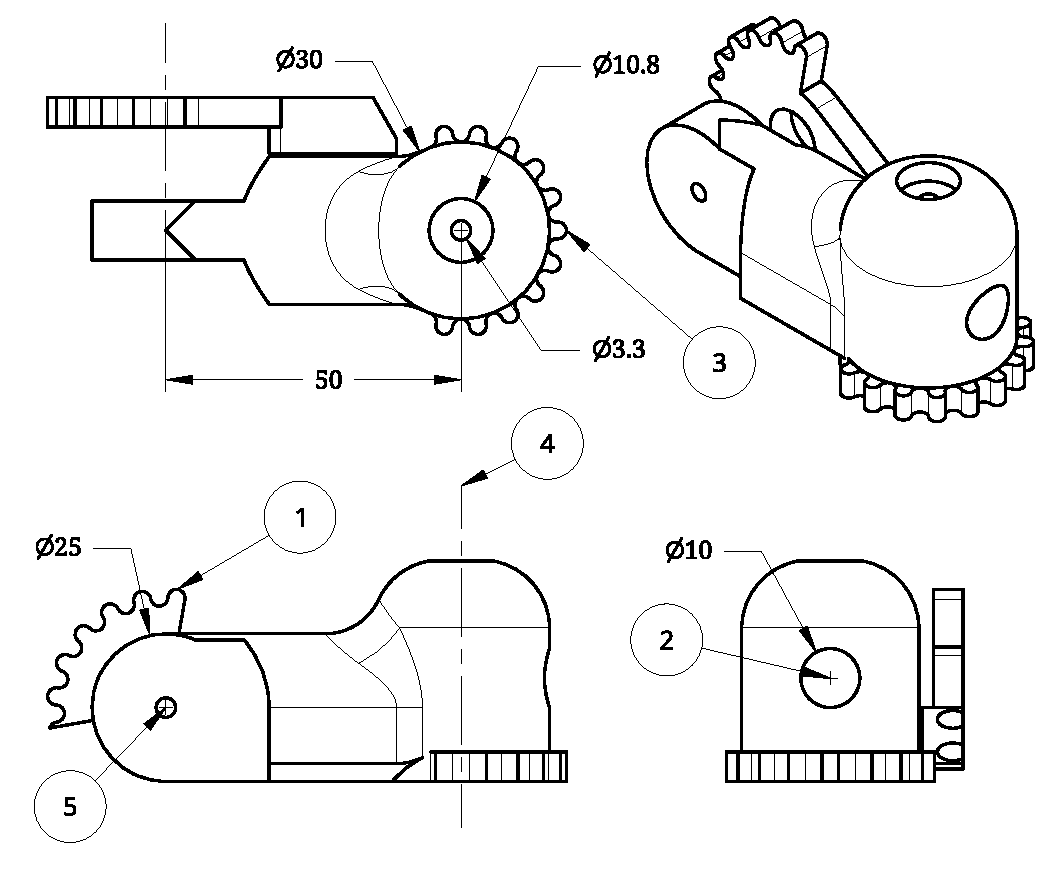
\includegraphics[scale = 0.8]{pics/DrawingA.pdf}
\caption{Illustration of how multiple servo motors are controlled using two timers.}
\label{fig:DrawingA}
\end{figure}

The annotations in Figure \ref{fig:DrawingB} that shows segment B is explained below:
\begin{enumerate}
\item Cavity for the servo motor that drives segment C.
\item Cavity for the servo motor that drives segment B.
\item Ball with slot that connects to segment A.
\item Peg that goes in the ball with slot in segment C.
\item Centreline where a stainless steel shaft is inserted into bearings for vertical movement with segment C.
\item Centreline where a stainless steel shaft is inserted into bearings for vertical movement with segment A.
\end{enumerate}

\begin{figure}[H]
\centering
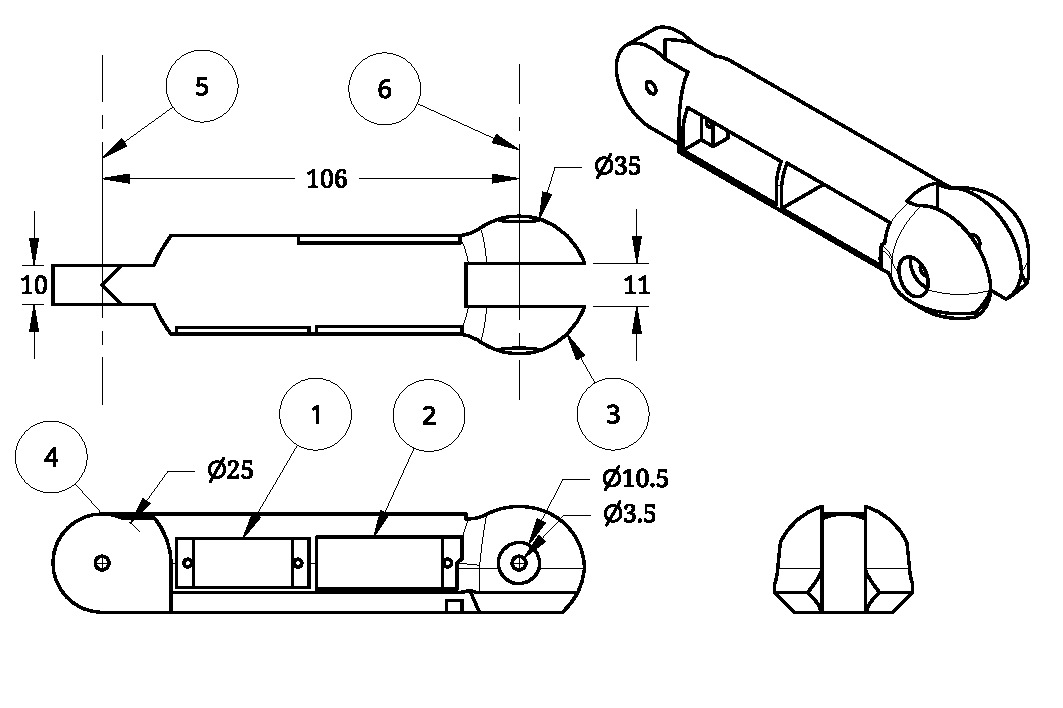
\includegraphics[scale = 0.8]{pics/DrawingB.pdf}
\caption{Illustration of how multiple servo motors are controlled using two timers.}
\label{fig:DrawingB}
\end{figure}

The annotations in Figure \ref{fig:DrawingC} that shows segment C is explained below:
\begin{enumerate}
\item Centreline where a stainless steel shaft is inserted into bearings for vertical movement with segment B.
\item Flat part of the foot that makes contact with the ground.
\item Cut-out that allows for a wider range of movement.
\end{enumerate}

\begin{figure}[H]
\centering
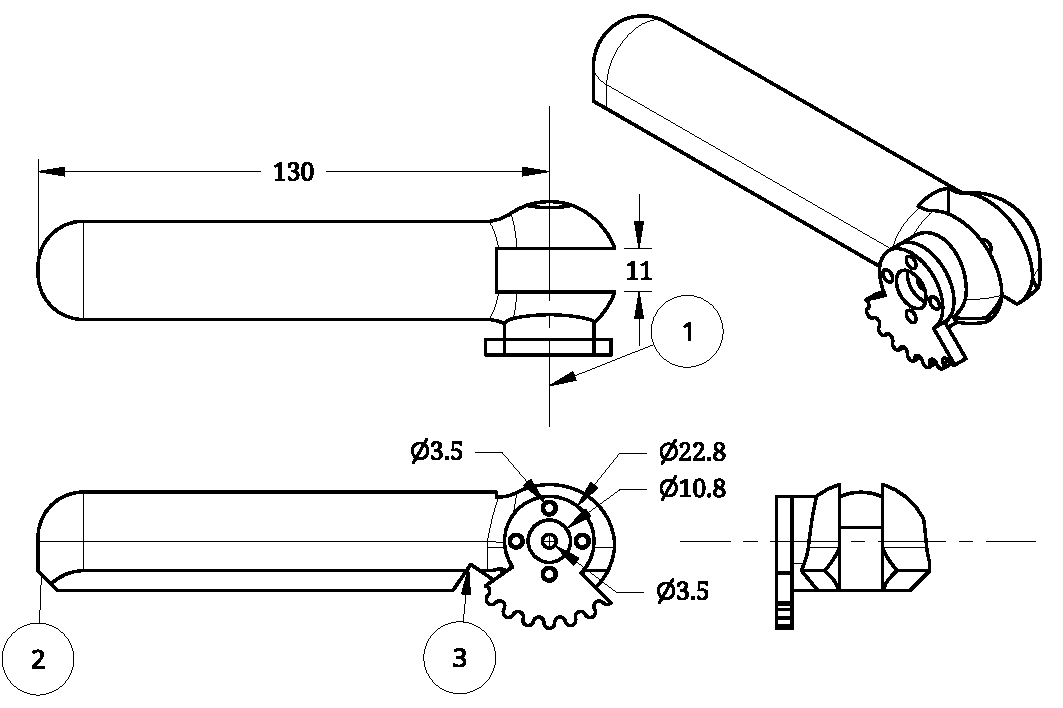
\includegraphics[scale = 0.8]{pics/DrawingC.pdf}
\caption{Illustration of how multiple servo motors are controlled using two timers.}
\label{fig:DrawingC}
\end{figure}

The annotations in Figure \ref{fig:DrawingBase} that shows the base is explained below:
\begin{enumerate}
\item Gear that connects to the servo motor located in leg B.
\item Hole for wire management.
\item Gear teeth that connect to the servo motor located in the base.
\item Centreline where a stainless steel shaft is inserted into bearings for horizontal movement.
\item Centreline where a stainless steel shaft is inserted into bearings for vertical movement.
\end{enumerate}

\begin{figure}[H]
\centering
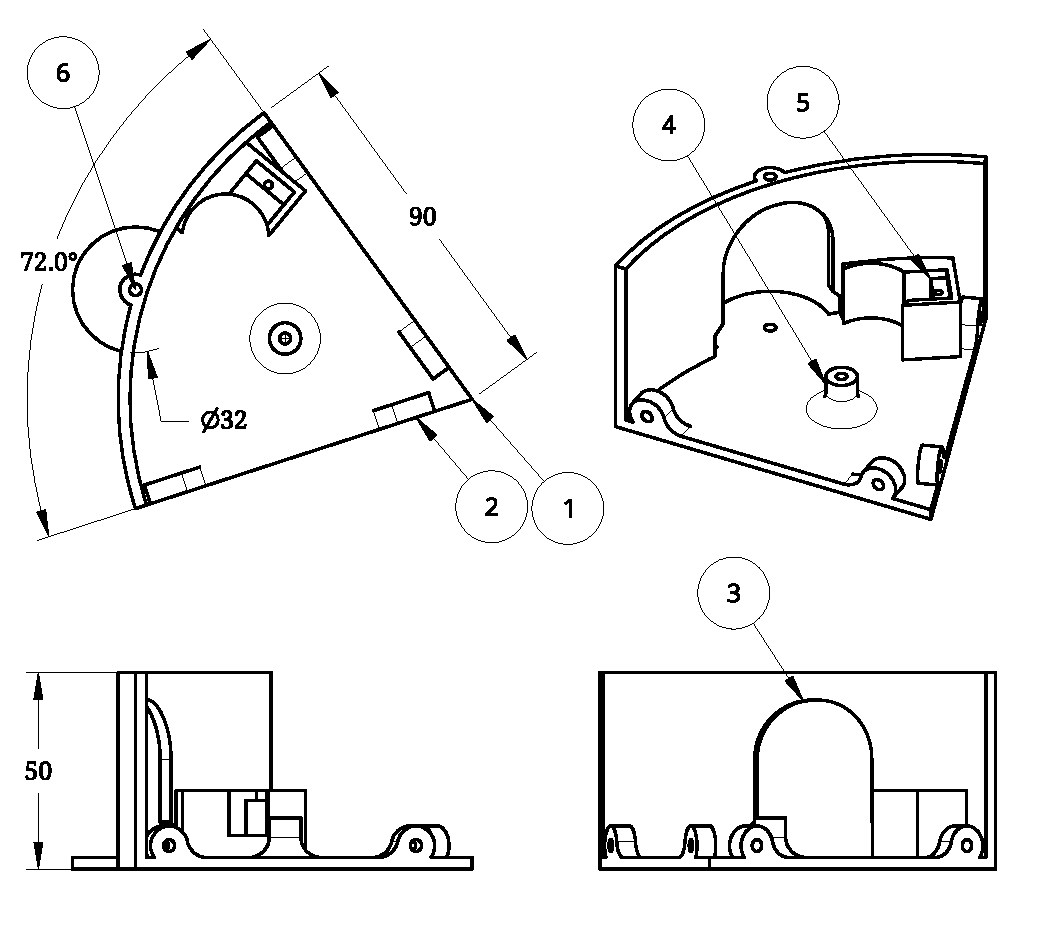
\includegraphics[scale = 0.8]{pics/DrawingBase.pdf}
\caption{Illustration of how multiple servo motors are controlled using two timers.}
\label{fig:DrawingBase}
\end{figure}

\subsubsection{Hardware implementation}

All of the hardware discussed above was 3D printed and assembled.\\

When the hardware was implemented, the servo motors we unable to lift the robot. A spiral torsion spring was designed and printed to help aid the lifting of the robot.\\

The annotations in Figure \ref{fig:DrawingSpring} that shows the torsion spring is explained below:
\begin{enumerate}
\item Hole for stainless steel shaft.
\item Mounting hub on servo gear.
\item Gear for servo.
\end{enumerate}

\begin{figure}[H]
\centering
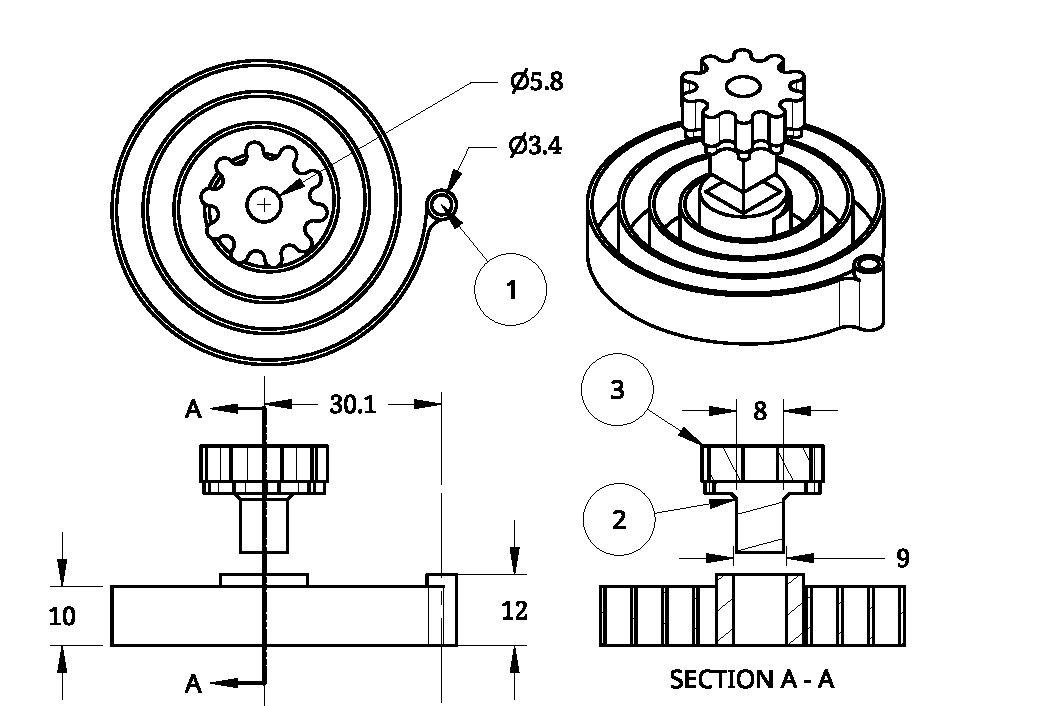
\includegraphics[scale = 0.8]{pics/DrawingSpring.pdf}
\caption{Illustration of how multiple servo motors are controlled using two timers.}
\label{fig:DrawingSpring}
\end{figure}